\documentclass[12pt]{article}

% Codificación y español
\usepackage[utf8]{inputenc}
\usepackage[T1]{fontenc}
\usepackage[spanish]{babel}

% Matemáticas
\usepackage{amsmath}
\usepackage{amssymb}

% Márgenes
\usepackage{geometry}
\geometry{margin=1in}

% Bibliografía
\usepackage[backend=biber,style=numeric]{biblatex}
\usepackage{csquotes}
\addbibresource{referenciasChallenge2.bib}

% Código
\usepackage{listings}
\usepackage{xcolor}
\usepackage{xurl}
\lstset{
    language=Python,
    basicstyle=\ttfamily\footnotesize,
    keywordstyle=\color{blue},
    commentstyle=\color{gray},
    stringstyle=\color{black},
    numbers=left,
    numberstyle=\tiny,
    frame=single,
    rulecolor=\color{black},
    breaklines=true,
    showstringspaces=false
}

% Imágenes y referencias
\usepackage{graphicx}
\usepackage{float}
\usepackage{hyperref}
\hypersetup{
    pdfborder={0 0 0}, % Elimina los rectángulos de colores
    colorlinks=true,   % Activa el color en el texto de la liga
    linkcolor=black,   % Color para referencias internas
    citecolor=black,   % Color para citas bibliográficas
    urlcolor=black     % Color para enlaces web
}

% Datos del documento
\title{Reto 2: New Shows and Movies - Netflix}
\author{Ing. Isaias Garcia Zanella}
\date{\today}

\begin{document}

\maketitle

\section{Introducción}

En el entorno actual de sobreabundancia informativa, la capacidad de transformar registros crudos en activos de conocimiento es fundamental para identificar tendencias y comportamientos de mercado. El presente reporte técnico detalla el análisis integral de un conjunto de datos compuesto por aproximadamente 8,800 registros de la plataforma Netflix, con el objetivo de caracterizar sus patrones de producción, distribución geográfica y preferencias de audiencia.

El desarrollo de este proyecto enfrentó desafíos críticos relacionados con la integridad de los datos. Se implementaron técnicas de extracción automatizada para la recuperación de metadatos en fuentes externas y se aplicaron mecanismos de imputación deductiva para mitigar el impacto de los valores faltantes en variables clave como el elenco y el país de origen. A través de una metodología analítica apoyada en herramientas de procesamiento estadístico, se exploraron dimensiones temporales y espaciales que revelan la transición de Netflix hacia un modelo de gestión basado en evidencia.

En este trabajo se busca dar respuesta a las siguientes interrogantes:
\begin{itemize}
    \item ¿Cómo varía la disponibilidad de contenido según la región geográfica?
    \item ¿Cuál ha sido la evolución del volumen de producción en los últimos 25 años?
    \item ¿Qué diferencias estructurales existen entre las series y las películas en términos de duración y audiencia?
    \item ¿Cuál es el periodo óptimo de lanzamiento para maximizar el impacto de una serie?
    \item ¿Quiénes son las figuras más prolíficas en la creación de contenido dentro de la plataforma?
\end{itemize}
\vspace{2cm}
\section{Marco Teórico}

\subsection{Datos faltantes}

Los datos faltantes son valores que no se encuentran disponibles dentro de un conjunto de datos. 
Estos pueden aparecer por diversas razones, como errores en la recopilación de información, 
problemas durante la integración de datos o simplemente porque la información no estaba 
disponible en el momento del registro.

La presencia de datos faltantes puede afectar significativamente el análisis estadístico y el desempeño de modelos de aprendizaje automático.

% \cite{Aceves2025IA}.

Diversos estudios han demostrado que los datos faltantes pueden introducir sesgos en los resultados 
del análisis si no se tratan adecuadamente. Por esta razón, el manejo correcto de valores ausentes 
es una etapa fundamental dentro del preprocesamiento de datos en proyectos de ciencia de datos 
y aprendizaje automático \cite{little2019missing}.

En la literatura se han identificado diferentes mecanismos mediante los cuales se presentan los 
datos faltantes. Entre los más comunes se encuentran los datos faltantes completamente al azar 
(\textit{Missing Completely At Random, MCAR}), los datos faltantes al azar (\textit{Missing At Random, MAR}) 
y los datos faltantes no al azar (\textit{Missing Not At Random, MNAR}). Comprender el tipo de 
mecanismo presente en el conjunto de datos permite seleccionar técnicas adecuadas para su tratamiento 
\cite{little2019missing}.

\subsection{Imputación con datos externos}

Las técnicas de imputación basadas en información externa o inferencia deductiva representan un enfoque
estratégico y dirigido para el tratamiento de valores faltantes. Estas técnicas se aplican cuando es posible deducir
los datos ausentes a partir de información contenida en otras instancias completas del conjunto de datos o mediante reglas lógicas
previamente definidas \cite{De0a100enIA}.

Dependiendo del problema que se tenga con los datos faltantes
se puede recuperar información adicional a partir de bases de datos, APIs 
o páginas web que contengan los datos necesarios.

En algunos casos, este proceso se realiza mediante técnicas de \textbf{web scraping}, donde se 
extrae información de sitios web para completar los valores faltantes en el conjunto de datos.

El uso de fuentes externas permite mejorar la calidad del conjunto de datos, ya que la información 
faltante puede recuperarse a partir de repositorios confiables o bases de datos públicas. Este 
enfoque resulta especialmente útil cuando se trabaja con conjuntos de datos incompletos obtenidos 
de diferentes fuentes o cuando la información puede ser verificada mediante múltiples recursos 
disponibles en internet \cite{hastie2009elements}.
\vspace{1.5cm}
\subsection{Web Scraping}

El \textit{web scraping} es una técnica utilizada para extraer información de páginas web de forma 
automatizada mediante programas o scripts. Esta técnica permite recopilar grandes volúmenes de 
información disponible en internet para su posterior análisis o almacenamiento en bases de datos 
\cite{mitchell2018webscraping}.

El proceso de web scraping generalmente consiste en enviar solicitudes a una página web, analizar 
la estructura del documento HTML recibido y localizar los elementos que contienen la información 
de interés. Posteriormente, estos datos pueden ser transformados y almacenados en formatos 
estructurados como archivos CSV, bases de datos o conjuntos de datos utilizados en análisis de 
datos \cite{mitchell2018webscraping}.

Actualmente, lenguajes de programación como Python ofrecen múltiples herramientas para realizar 
web scraping, entre las que destacan bibliotecas como \textit{BeautifulSoup}, \textit{Scrapy} y 
\textit{Selenium}, las cuales facilitan la extracción y procesamiento de información contenida en 
sitios web.

\subsection{Netflix}

Netflix es una plataforma de streaming que ofrece una amplia variedad de series, películas, 
documentales y programas de entretenimiento. La plataforma ha generado grandes volúmenes de 
datos relacionados con su catálogo de contenido, los cuales pueden ser utilizados para realizar 
análisis de datos, recomendaciones y estudios de tendencias de consumo.

Debido a la gran cantidad de contenido disponible en la plataforma, Netflix ha sido un caso de 
estudio frecuente en investigaciones relacionadas con sistemas de recomendación, minería de datos 
y análisis de comportamiento de usuarios \cite{gomez2016netflix}.

El análisis de estos datos permite aplicar técnicas de ciencia de datos y aprendizaje automático 
para identificar patrones de consumo y mejorar la experiencia de los usuarios mediante sistemas 
de recomendación personalizados \cite{russell2021ai}.

\vspace{6cm}
\section{Materiales y Métodos}

\subsection{Materiales}

Para el desarrollo de la presente actividad se configuró un ecosistema de trabajo basado en hardware de alto rendimiento y software especializado para ciencia de datos:

\begin{itemize} 
    \item \textbf{Equipo:} Laptop HP Victus con arquitectura de alto desempeño.
    \item \textbf{Procesador:} AMD Ryzen 7000 Series.
    \item \textbf{Tarjeta gráfica:} NVIDIA GeForce RTX 4050.
    \item \textbf{Lenguaje:} Python 3.x.
    \item \textbf{IDE:} Visual Studio Code (VS Code).
    \item \textbf{Kernel:} Jupyter Notebook.
    \item \textbf{Gestor de entorno:} Anaconda (Conda).
    \item \textbf{Bibliotecas:} \texttt{Pandas}, \texttt{Matplotlib} y \texttt{Seaborn}.
    \item \textbf{Base de datos:} 
    \\ \url{https://github.com/marcoaaceves/DataScience/blob/main/New%20Movies%20Netflix%20Data%20Exploration/netflix_data.csv}
\end{itemize}

\section{Métodos}

En esta sección se describe el proceso seguido para la obtención, limpieza y 
completado de los datos faltantes utilizando técnicas de \textit{web scraping}. 
El objetivo principal fue recuperar información faltante de un conjunto de datos 
relacionado con el catálogo de contenido de Netflix.

\subsection{Funciones implementadas}

Para el desarrollo del proyecto se implementaron diversas funciones en Python con el objetivo
de automatizar el proceso de carga de datos, obtención de información mediante web scraping,
análisis del conjunto de datos y generación de visualizaciones.

\subsubsection{Carga del conjunto de datos}

La función \texttt{load\_data\_local} permite cargar un archivo CSV utilizando la biblioteca
\texttt{pandas}. En caso de que ocurra algún error durante la lectura del archivo, la función
muestra un mensaje indicando el problema.

\begin{lstlisting}
def load_data_local(ubicacion):
    try:
        df = pd.read_csv(ubicacion)
        return df
    except Exception as e:
        print(f"Error al cargar la B.D.: {e}")
        return None
\end{lstlisting}

\subsubsection{Extracción de información desde Rotten Tomatoes}

La función \texttt{extraer\_rotten\_tomatoes} realiza una búsqueda del título de una película
o serie dentro del sitio web Rotten Tomatoes. Posteriormente analiza el contenido HTML de la
página para obtener información relevante como el director y parte del elenco.

\begin{lstlisting}
def extraer_rotten_tomatoes(titulo, session):
    try:
        search_url = f"https://www.rottentomatoes.com/search?search={titulo.replace(' ', '%20')}"
        res_search = session.get(search_url, timeout=10)
        soup_search = BeautifulSoup(res_search.text, 'html.parser')
        
        resultado = soup_search.find('a', {'data-qa': 'info-name'})
        if not resultado:
            return None
            
        url_final = resultado['href']
        res_page = session.get(url_final, timeout=10)
        soup_page = BeautifulSoup(res_page.text, 'html.parser')
        
        director = "N/A"
        dir_label = soup_page.find('b', string=lambda s: s and 'Director' in s)
        if dir_label:
            director = dir_label.find_next('span').text.strip()
            
        cast_items = soup_page.find_all('p', {'data-qa': 'cast-crew-item-name'})
        cast_final = ", ".join([actor.text.strip() for actor in cast_items[:3]])

        return {
            "pais": "",
            "director": director,
            "cast": cast_final
        }
    except Exception:
        return None
\end{lstlisting}

\subsubsection{Extracción de información desde IMDb}

La función \texttt{extraer\_imdb} realiza una búsqueda del título dentro del sitio web IMDb.
Posteriormente obtiene información estructurada del contenido utilizando datos en formato
JSON incrustados en la página, lo que permite recuperar datos como el director, el elenco
principal y el país de origen.

\begin{lstlisting}
def extraer_imdb(titulo, session):
    try:
        search_url = f"https://www.imdb.com/find?q={titulo.replace(' ', '+')}"
        res_search = session.get(search_url, timeout=10)
        soup_search = BeautifulSoup(res_search.text, 'html.parser')

        resultado = soup_search.find('a', href=lambda h: h and '/title/tt' in h)
        if not resultado:
            return None

        url_final = f"https://www.imdb.com{resultado['href'].split('?')[0]}"
        res_page = session.get(url_final, timeout=10)
        soup_page = BeautifulSoup(res_page.text, 'html.parser')

        script_tag = soup_page.find('script', type='application/ld+json')
        data = json.loads(script_tag.string) if script_tag else {}

        directores = data.get("director", []) or data.get("creator", [])
        if isinstance(directores, list):
            director_final = ", ".join([d.get("name") for d in directores if "name" in d])
        else:
            director_final = directores.get("name") if directores else ""

        reparto = data.get("actor", [])
        cast_final = ", ".join([a.get("name") for a in reparto[:3]])

        return {
            "pais": "",
            "director": director_final,
            "cast": cast_final
        }

    except Exception:
        return None
\end{lstlisting}
\vspace{2cm}
\subsubsection{Proceso principal de Web Scraping}

La función \texttt{Web\_Scrapping\_Pro} coordina el proceso completo de recuperación de
información faltante. Esta función recorre cada registro del conjunto de datos y, cuando
detecta valores faltantes en las columnas de país, director o elenco, intenta obtener
dicha información desde IMDb o Rotten Tomatoes.

\begin{lstlisting}
def Web_Scrapping_Pro(dataSet):

    session = requests.Session()

    for i, fila in dataSet.iterrows():

        if not ((pd.isna(fila['country']) or fila['country'] == "") and 
                (pd.isna(fila['cast']) or fila['cast'] == "") and 
                (pd.isna(fila['director']) or fila['director'] == "")):
            continue

        titulo_busqueda = fila.get('title', '')

        datos_extraidos = extraer_imdb(titulo_busqueda,session)

        if not datos_extraidos:
            datos_extraidos = extraer_rotten_tomatoes(titulo_busqueda,session)

        if datos_extraidos:
            dataSet.at[i, 'country'] = datos_extraidos.get('pais', '')
            dataSet.at[i, 'director'] = datos_extraidos.get('director', '')
            dataSet.at[i, 'cast'] = datos_extraidos.get('cast', '')

    return dataSet
\end{lstlisting}

\subsubsection{Funciones auxiliares}

Además del proceso de web scraping, se implementaron funciones auxiliares
para realizar operaciones de análisis dentro del conjunto de datos.

\begin{lstlisting}
def get_max_value(values):
    max_val = None
    for p in values:
        if max_val is None or (isinstance(p,(int,float)) and p > max_val):
            max_val = p
    return max_val
\end{lstlisting}

\begin{lstlisting}
def get_min_value(values): 
    min_value = None
    for p in values:
        if min_value is None or (isinstance(p,(int,float)) and p < min_value):
            min_value = p
    return min_value
\end{lstlisting}
\vspace{1cm}
\subsubsection{Funciones de análisis del dataset}

También se desarrollaron funciones que permiten filtrar el tipo de contenido
(películas o series) y realizar distintos tipos de análisis sobre el conjunto
de datos.

\begin{lstlisting}
def filtrar_Tipo(df, tipo):
    opciones = {1: 'Movie', 2: 'TV Show'}
    return df[df['type'] == opciones.get(tipo, 'Movie')]
\end{lstlisting}

Estas funciones permiten organizar el conjunto de datos de acuerdo con el tipo
de contenido y facilitan la generación de análisis estadísticos y visualizaciones
posteriores.


\section{Resultados y Discusión}
Como se mencionó en la sección de introducción, en este apartado se presentan los resultados obtenidos
a partir de las preguntas planteadas inicialmente. Asimismo, se realiza una explicación de dichos
resultados con el objetivo de que el cliente pueda comprenderlos de manera clara y facilitar así
la toma de decisiones.
\subsection{¿Qué tipo de contenido está disponible en diferentes países?}

La gráfica resultante se muestra a continuación:
\begin{figure}[H]
    \centering
    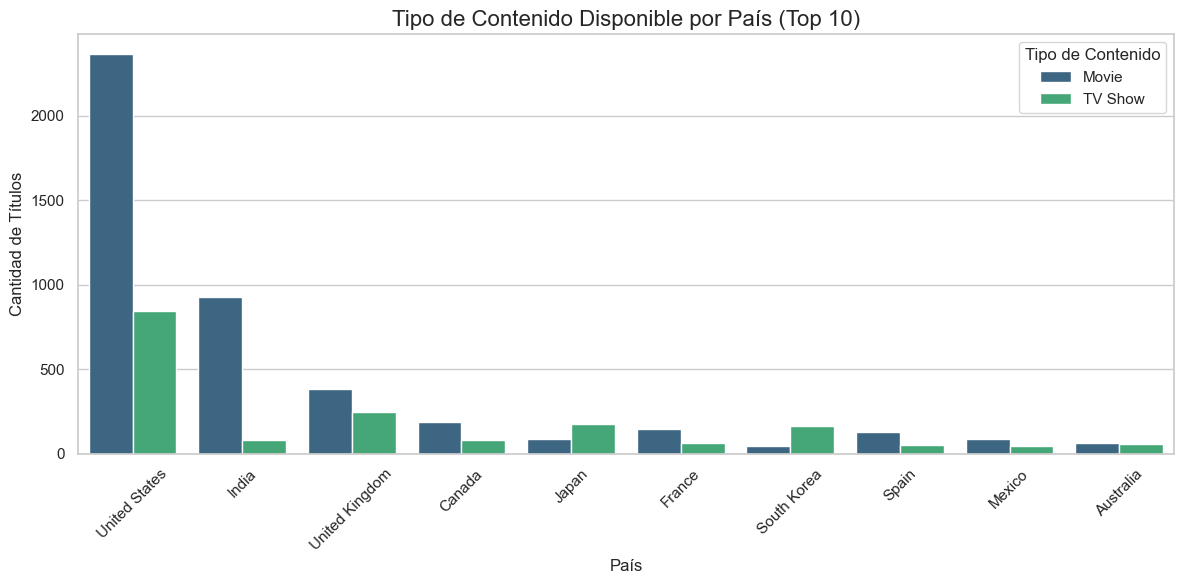
\includegraphics[width=0.75\linewidth]{../Imagenes/Reto_2/Contenido_Disponible_Paises.png}
    \caption{Tipo de contenido disponible por pais.}
    \label{fig:contenido_paises}
\end{figure}

A partir de la Figura \ref{fig:contenido_paises}, se puede observar que Estados Unidos
es el país con mayor cantidad de contenido disponible en la plataforma, tanto en
películas como en series de televisión. Esto sugiere que gran parte del catálogo
de Netflix está dominado por producciones provenientes de este país.

Asimismo, países como India y Reino Unido también presentan una cantidad considerable
de contenido, principalmente en la categoría de películas. Por otro lado, países
como Japón y Corea del Sur muestran una presencia importante de series de televisión,
lo cual puede estar relacionado con la popularidad de sus producciones televisivas
en el mercado internacional.

\subsection{¿Cuanto es el numero de peliculas o tv shows que salieron han cambiado en los ultimos years? 20 - 30 }

A continuación, se presenta la evolución del volumen de contenidos producidos anualmente en los últimos 25 años, segmentados por tipo de producción (\textit{Movie} y \textit{TV Show}):

\begin{figure}[H]
    \centering
    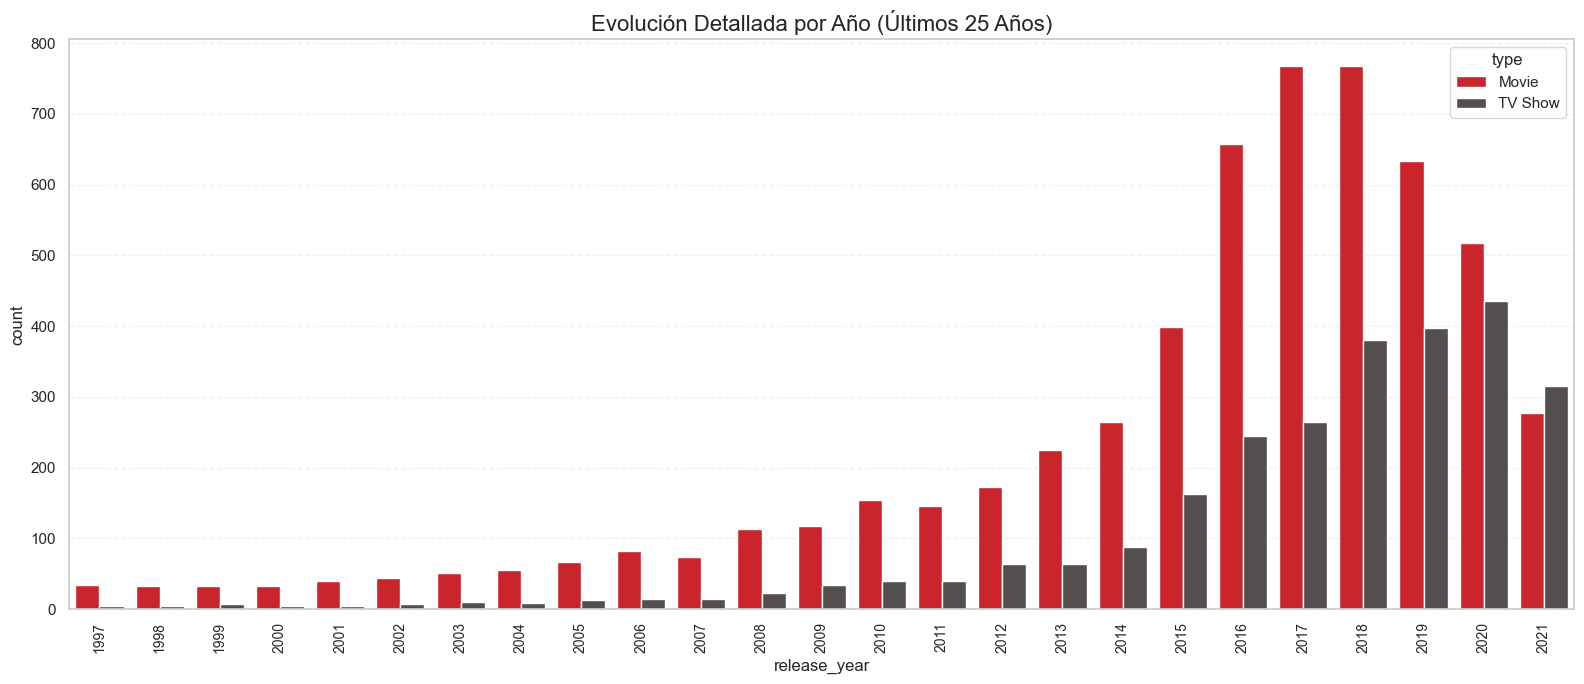
\includegraphics[width=0.95\linewidth]{../Imagenes/Reto_2/Contenido_Subido_25 years.png}
    \caption{Evolución detallada del contenido por año de lanzamiento (1997-2021).}
    \label{fig:evolucion_temporal}
\end{figure}

A partir de la Figura \ref{fig:evolucion_temporal}, se identifican tres fases críticas en la estrategia de adquisición de la plataforma:

\begin{itemize}
    \item \textbf{Estabilidad Inicial (1997--2012):} Durante este periodo, el crecimiento del catálogo fue moderado y lineal, con una predominancia casi absoluta de largometrajes y una presencia marginal de series de televisión.
    \item \textbf{Fase de Expansión Exponencial (2013--2018):} Se observa un incremento disruptivo en la cantidad de películas, alcanzando picos superiores a los 750 títulos anuales en 2017 y 2018. Este fenómeno coincide con la transición de Netflix hacia la producción masiva de contenido original para reducir la dependencia de licencias externas.
    \item \textbf{Pivotaje Estratégico (2019--2021):} Se detecta un cambio significativo en el modelo de negocio. Mientras que la producción de películas muestra un descenso tras su pico en 2018, los \textit{TV Shows} mantienen una tendencia ascendente, llegando a superar el volumen de películas en el año 2021.
\end{itemize}

Este comportamiento sugiere una transición estratégica hacia la retención de usuarios mediante formatos episódicos, los cuales fomentan un \textit{engagement} a largo plazo y una recurrencia mayor en la suscripción en comparación con los largometrajes de consumo único.

\section{Análisis Comparativo: Películas vs. Series de TV}

El análisis del catálogo permite diferenciar las estrategias de contenido mediante tres dimensiones: la madurez de la audiencia (Rating), la estructura de consumo (Duración) y la tendencia histórica de crecimiento.

\subsection{Clasificación por Audiencias (Rating)}

En la Figura \ref{fig:rating_comp}, se observa la distribución de los títulos según su clasificación de madurez. Es evidente que tanto en películas como en series, la categoría \textbf{TV-MA} (para adultos) es la predominante.

\begin{figure}[H]
    \centering
    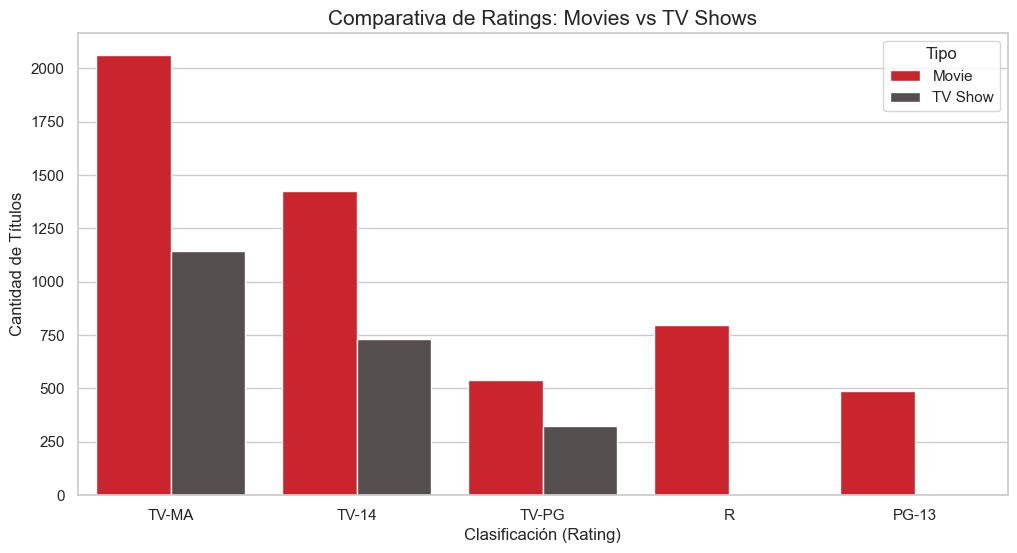
\includegraphics[width=0.85\linewidth]{../Imagenes/Reto_2/Comparativa_Rating_vs.png}
    \caption{Comparativa de Ratings: Dominio de contenido para audiencias adultas.}
    \label{fig:rating_comp}
\end{figure}

\textbf{Interpretación:} El alto volumen de contenido TV-MA sugiere que la propuesta de valor de Netflix se centra en dramas complejos y producciones maduras, buscando atraer a un sector demográfico con mayor capacidad de retención y discusión en plataformas digitales.

\subsection{Estructura de Consumo: Duración y Temporadas}

Para entender cómo se consume el contenido, es necesario contrastar la duración de los largometrajes frente a la longevidad de las series. Las Figuras \ref{fig:duracion} y \ref{fig:temporadas} representan este comportamiento:

\begin{figure}[H]
    \centering
    % Primera imagen: Duración de Películas
    \begin{minipage}{0.48\textwidth}
        \centering
        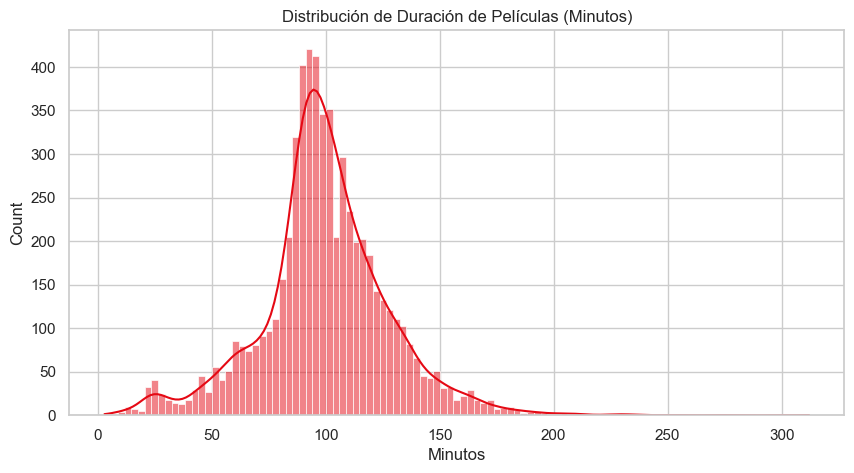
\includegraphics[width=\linewidth]{../Imagenes/Reto_2/PeliculavsShows_Duracion.png}
        \caption{Distribución de duración en minutos (Películas).}
        \label{fig:duracion}
    \end{minipage}\hfill
    % Segunda imagen: Distribución de Temporadas
    \begin{minipage}{0.48\textwidth}
        \centering
        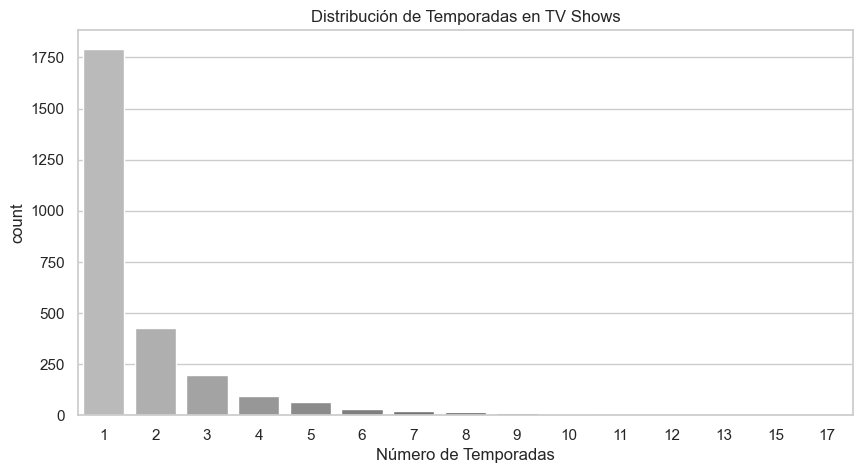
\includegraphics[width=\linewidth]{../Imagenes/Reto_2/Distribucion Temporadas_tvShows.png}
        \caption{Distribución de temporadas (TV Shows).}
        \label{fig:temporadas}
    \end{minipage}
\end{figure}

\textbf{Análisis Técnico:} 
\begin{itemize}
    \item \textbf{Películas:} Presentan una distribución unimodal con un pico claro entre los 90 y 110 minutos, lo que indica un estándar de industria para maximizar el visionado completo.
    \item \textbf{Series:} Existe un sesgo masivo hacia series de una sola temporada. Esto refleja una estrategia de "lanzamiento y filtrado", donde la plataforma produce una gran variedad de pilotos o series limitadas, renovando únicamente aquellas que logran métricas de éxito excepcionales.
\end{itemize}

\subsection{Evolución Histórica (Últimos 25 años)}

Finalmente, la Figura \ref{fig:evolucion_temporal} muestra cómo ha cambiado el volumen de lanzamientos anuales, marcando la transición de un servicio de renta a una potencia de producción original.
\\
\textbf{Conclusión:} Se identifica un hito estratégico entre 2018 y 2021. Mientras las películas alcanzaron su saturación, las series continuaron su ascenso, superando en volumen a los largometrajes hacia el final del periodo. Esto confirma el enfoque actual de la compañía: \textbf{invertir en contenido episódico para garantizar suscripciones recurrentes}.

\subsection{¿Cuando es el mejor momento para lanzar una serie de television?}

Para determinar el momento estratégico ideal para el lanzamiento de una serie de televisión, se analizó la distribución porcentual de estrenos por mes a lo largo del histórico disponible.

\begin{figure}[H]
    \centering
    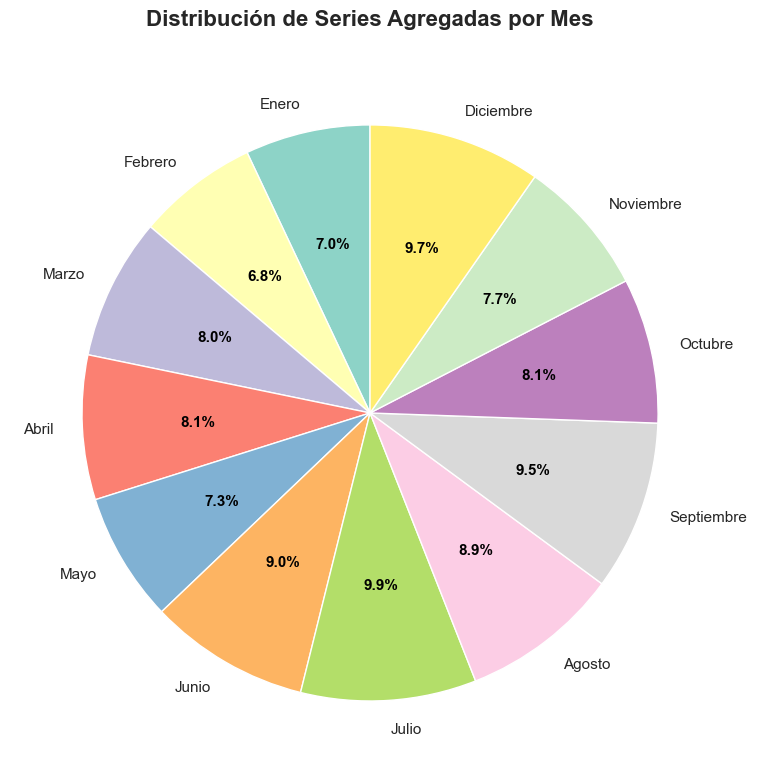
\includegraphics[width=0.7\linewidth]{../Imagenes/Reto_2/SeriesAgregadas_por_Mes.png}
    \caption{Distribución porcentual de series agregadas por mes.}
    \label{fig:mes_lanzamiento}
\end{figure}

A partir de la Figura \ref{fig:mes_lanzamiento}, se desprenden las siguientes observaciones técnicas sobre el comportamiento de la plataforma:

\begin{itemize}
    \item \textbf{Concentración en Periodos de Alta Demanda:} Los meses con mayor volumen de lanzamientos son \textbf{Julio (9.9\%)} y \textbf{Diciembre (9.7\%)}. Esta tendencia sugiere una planificación orientada a capturar la atención del usuario durante los periodos vacacionales de verano e invierno, donde el tiempo de visionado (\textit{watch time}) tiende a incrementarse globalmente.
    \item \textbf{Valles de Publicación:} Los meses de \textbf{Enero (7.0\%)} y \textbf{Febrero (6.8\%)} presentan la menor actividad. Desde una perspectiva de marketing digital, estos meses representan un ``océano azul'' donde la competencia interna por el algoritmo de recomendación es menor, permitiendo una mayor visibilidad para producciones nuevas.
    \item \textbf{Relación con el Ciclo de Renovación:} Dado que la mayoría de los \textit{TV Shows} cuentan con una sola temporada, los lanzamientos en el tercer trimestre (Q3) permiten recolectar suficientes métricas de \textit{engagement} para informar las decisiones de renovación antes del cierre del año fiscal.
\end{itemize}

\textbf{Conclusión Estratégica:} El mejor momento para el lanzamiento depende del objetivo de negocio. Para maximizar el alcance masivo, los meses de \textbf{Julio y Septiembre} son óptimos debido al tráfico orgánico. No obstante, para producciones de nicho que requieran destacar sin la interferencia de grandes \textit{blockbusters}, el primer trimestre del año ofrece una ventana de menor saturación en el catálogo.

\subsection{Análisis de Talento: Actores y Directores más Prolíficos}

Un hallazgo contundente en el análisis del catálogo es la discrepancia entre el país con mayor volumen de contenido (Estados Unidos) y el origen de los individuos con mayor cantidad de participaciones en la plataforma.

\begin{figure}[H]
    \centering
    \begin{minipage}{0.48\textwidth}
        \centering
        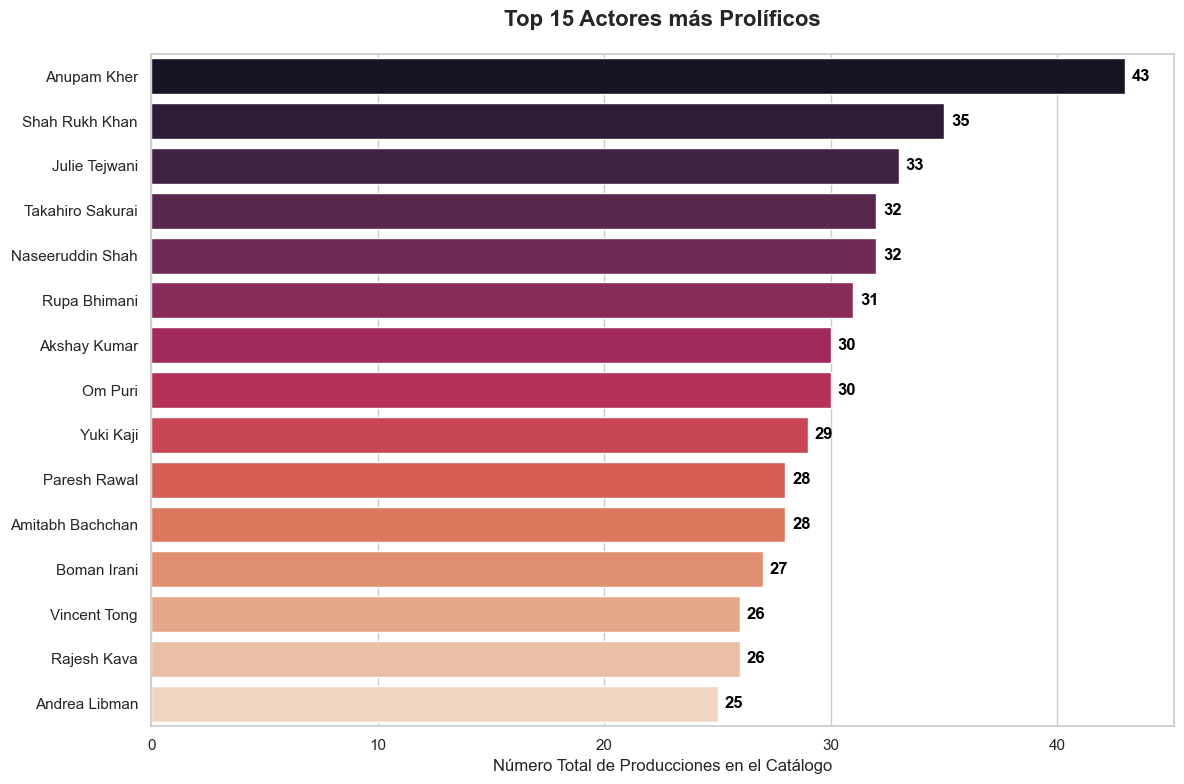
\includegraphics[width=\linewidth]{../Imagenes/Reto_2/Top15Actores.png}
        \caption{Top 15 Actores con más títulos.}
        \label{fig:top_actores}
    \end{minipage}\hfill
    \begin{minipage}{0.48\textwidth}
        \centering
        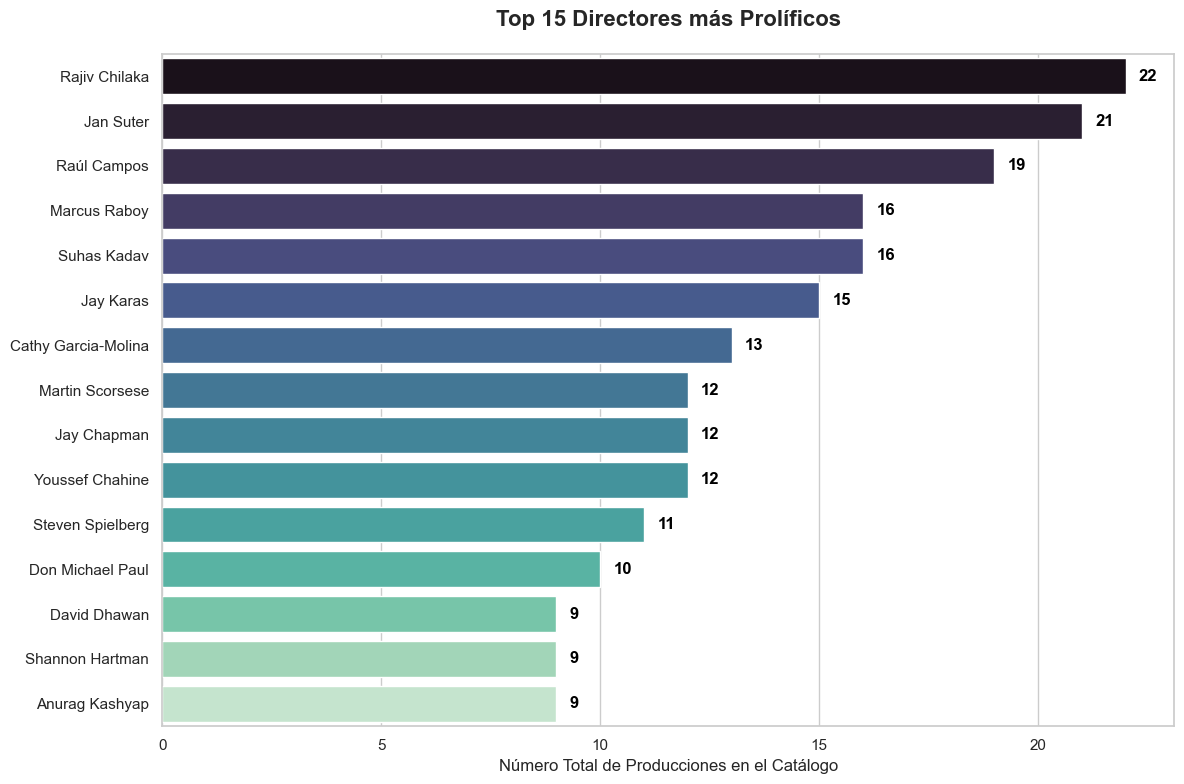
\includegraphics[width=\linewidth]{../Imagenes/Reto_2/Top15Directores.png}
        \caption{Top 15 Directores con más títulos.}
        \label{fig:top_directores}
    \end{minipage}
\end{figure}

A partir de las Figuras \ref{fig:top_actores} y \ref{fig:top_directores}, se desprenden las siguientes conclusiones técnicas:

\begin{itemize}
    \item \textbf{Predominio de la Industria de la India:} A pesar del dominio geográfico de EE. UU. en el dataset global, el \textit{ranking} de actores está liderado casi en su totalidad por figuras de la India. \textbf{Anupam Kher} encabeza la lista con 43 producciones, seguido de \textbf{Shah Rukh Khan} (35) y \textbf{Naseeruddin Shah} (32). Este fenómeno se explica por la estructura de producción de Bollywood, caracterizada por una alta rotación de talento en un volumen masivo de cintas anuales.
    \item \textbf{Diversidad en el Talento Vocal:} Destaca la presencia de actores como \textbf{Julie Tejwani} y \textbf{Takahiro Sakurai}, lo que sugiere un peso importante de las producciones de animación y doblaje (tanto de India como de Japón) en la oferta de contenido recurrente.
    \item \textbf{Liderazgo en Dirección:} En la dirección, \textbf{Rajiv Chilaka} lidera con 22 títulos, impulsado principalmente por el éxito de franquicias de animación. Le siguen directores enfocados en el mercado latinoamericano y de comedia, como \textbf{Jan Suter} y \textbf{Raúl Campos} (19-21 títulos), lo que refuerza la estrategia de Netflix de adquirir catálogos completos de directores prolíficos para mercados específicos.
\end{itemize}

\textbf{Interpretación de Negocio:} Para Netflix, estos actores y directores representan un pilar de contenido de alta fidelidad. Aunque Estados Unidos produce más variedad, el talento de la India y los mercados de animación generan una densidad de contenido que permite mantener bibliotecas robustas con figuras familiares para audiencias globales masivas.

\subsection{Distribución Geográfica: ¿Qué tipo de contenido está disponible en diferentes países?}

El alcance global de Netflix se manifiesta de manera heterogénea a través de los diversos mercados internacionales. Para analizar esta distribución sin que los valores atípicos de regiones con alta producción saturaran la visualización, se aplicó una transformación logarítmica a los datos, permitiendo una comparativa más equilibrada entre naciones.

\begin{figure}[H]
    \centering
    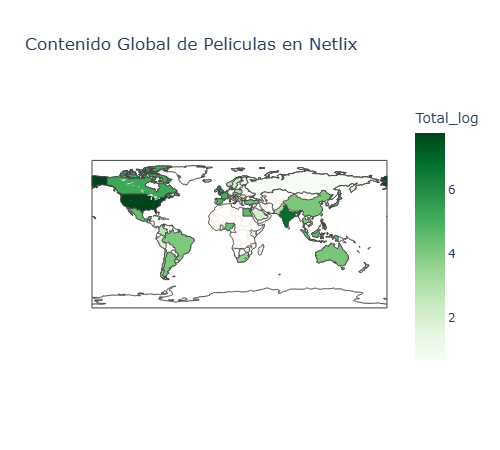
\includegraphics[width=0.85\linewidth]{../Imagenes/Reto_2/Contenido_global.png}
    \caption{Distribución global de contenido por país (Escala Logarítmica).}
    \label{fig:contenido_global}
\end{figure}

A partir de la Figura \ref{fig:contenido_global}, se pueden extraer las siguientes conclusiones sobre la disponibilidad de contenido:

\begin{itemize}
    \item \textbf{Hegemonía de Estados Unidos:} Como se observa en la coloración más intensa del mapa, Estados Unidos se consolida como el principal exportador de contenido, dominando el catálogo tanto en volumen de películas como de series de televisión. Esto refleja no solo el origen de la plataforma, sino la centralización de la industria cinematográfica global en Hollywood.
    \item \textbf{Especialización en Mercados Asiáticos:} Países como \textbf{Japón} y \textbf{Corea del Sur} presentan una densidad considerable de contenido, con una marcada especialización en el formato de \textit{TV Shows}. El éxito global del \textit{Anime} y los \textit{K-Dramas} ha convertido a estas regiones en pilares fundamentales para la retención de usuarios interesados en narrativas episódicas.
    \item \textbf{Potencia Cinematográfica de la India:} India destaca como el segundo mayor productor en el dataset, con un enfoque masivo en largometrajes. A diferencia de los mercados occidentales, la producción de Bollywood mantiene una rotación de contenido muy alta, lo que se traduce en una presencia dominante en la categoría de películas.
    \item \textbf{Mercados Emergentes y Conectividad:} Regiones como Reino Unido, Canadá y Francia actúan como nodos secundarios importantes, a menudo participando en coproducciones internacionales que enriquecen la diversidad lingüística del catálogo.
\end{itemize}

\textbf{Análisis de Ingeniería:} La implementación de la escala logarítmica en la visualización fue crucial para identificar que, si bien el volumen total es liderado por EE. UU., la presencia de Netflix es verdaderamente global, con centros de producción activos en todos los continentes que alimentan el algoritmo de recomendación de manera diversificada.

\section{Conclusión}

Después de analizar los datos del catálogo de Netflix, se han identificado tres puntos clave que explican cómo funciona su contenido actualmente:

\begin{itemize}
    \item \textbf{Más series que películas:} Los datos muestran que, a partir de 2018, Netflix empezó a dar prioridad a las series sobre las películas. Esto se debe a que las series mantienen a la gente usando la plataforma por más tiempo.
    \item \textbf{Dominio de EE. UU. e India:} Aunque Estados Unidos tiene la mayor cantidad de títulos, India es la que tiene a los actores y directores más productivos. Esto demuestra que la industria de la India es una pieza fundamental para llenar el catálogo de la plataforma.
    \item \textbf{Especialización por país:} El análisis reveló que cada región tiene su fuerte; por ejemplo, mientras India destaca en películas, Japón y Corea del Sur son líderes en series de televisión (animación y dramas).
\end{itemize}

En resumen, el éxito de Netflix no solo se debe a la cantidad de videos que tiene, sino a que sabe qué tipo de contenido producir en cada país y en qué meses lanzarlos para aprovechar las épocas de vacaciones.
\printbibliography[title={Referencias bibliográficas}]

\end{document}